\usetikzlibrary{arrows.meta}
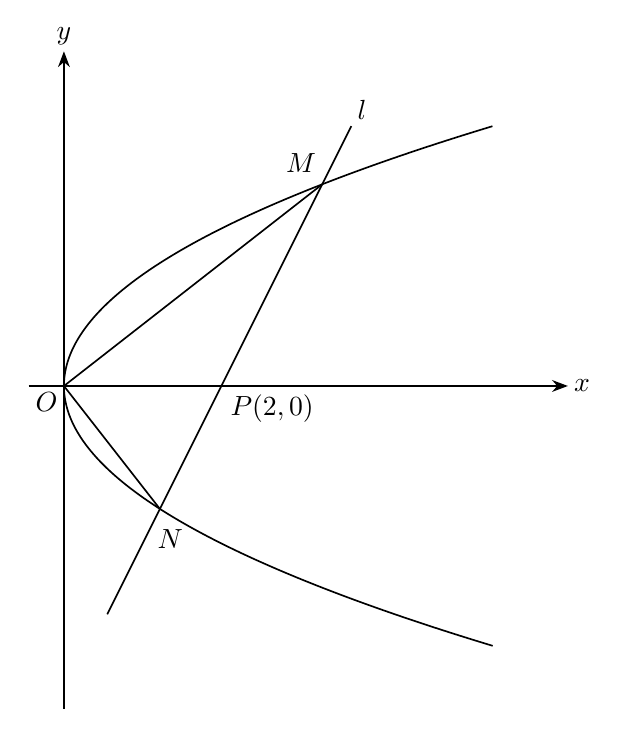
\begin{tikzpicture}[x=1cm,y=1cm,line width=.6pt,>=Stealth,font=\normalsize]
\coordinate (O) at (0,0);
\coordinate (P) at (2,0);
\coordinate (M) at (3.2808,2.5616);
\coordinate (N) at (1.2192,-1.5616);
\coordinate (L0) at (0.55,-2.9);
\coordinate (L1) at (3.65,3.3);
\coordinate (X0) at (-0.45,0);
\coordinate (X1) at (6.4,0);
\coordinate (Y0) at (0,-4.1);
\coordinate (Y1) at (0,4.25);
\coordinate (NL) at (1.35,-1.81);
\draw[->] (X0) -- (X1);
\draw[->] (Y0) -- (Y1);
\draw[domain=-3.3:3.3,samples=161,smooth,variable=\t] plot ({\t*\t/2},{\t});
\draw (L0) -- (L1);
\draw (O) -- (M);
\draw (O) -- (N);
\node[anchor=north east,inner sep=0pt,xshift=-2pt,yshift=-2pt] at (O) {$O$};
\node[anchor=north west,inner sep=0pt,xshift=3pt,yshift=-3pt] at (P) {$P(2,0)$};
\node[anchor=south east,inner sep=0pt,xshift=-2pt,yshift=4pt] at (M) {$M$};
\node[anchor=north,inner sep=0pt] at (NL) {$N$};
\node[anchor=south west,inner sep=0pt,xshift=2pt,yshift=2pt] at (L1) {$l$};
\node[anchor=west,inner sep=0pt,xshift=2pt] at (X1) {$x$};
\node[anchor=south,inner sep=0pt,yshift=2pt] at (Y1) {$y$};
\end{tikzpicture}
